%% The following is a directive for TeXShop to indicate the main file
%%!TEX root = diss.tex

\chapter{Preliminaries}
\label{ch:Preliminaries}

We outline a number of existing techniques, methods, and algorithms relevant to augmenting metadata, we show how metadata augmentation can be accomplished after modifications are made to the techniques, methods, and algorithms. We first discuss semantic enrichment in \autoref{sec:SemanticEnrichment}, where a dictionary definition is attached to each word of the attributes and tags. We next discuss the schema matching algorithm in \autoref{sec:SchemaMatching}; the idea of matching will be used throughout the other algorithms we introduce. We next discuss semantic labeling in \autoref{sec:SemanticLabeling}, where each of the attributes is labeled with a tag. The base table of the metadata augmentation problem is related to each of the tables by a table search algorithm we introduce in \autoref{sec:FindingRelatednessBetweenTables}. We finally discuss a partitioning algorithm in \autoref{sec:Partitioning} to group similar attributes and similar tags together. We use the word \textit{algorithm} when explaining something in a fine-grained manner, we use the words \textit{method} and \textit{technique} interchangeably when explaining some matter without going into its details.

%%%%%%%%%%%%%%%%%%%%%%%%%%%%%%%%%%%%%%%%%%%%%%%%%%%%%%%%%%%%%%%%%%%%%%
\section{Semantic enrichment}
\label{sec:SemanticEnrichment}

In Surrey Open Data in \autoref{fig:example-parks}, the word \textit{park} in the header \textit{park name}, according to a domain dictionary, could be interpreted as `amusement parks', `an open green space', or even a `parking lot'. Which interpretation is the correct one? The \textit{table name} does not provide any additional information, neither does the \textit{table description}. However, the \textit{category} and the \textit{tags} contain useful information that we can use to disambiguate the word. The \textit{category} contains the word \textit{environment} while the \textit{tags} contain words \textit{green} and \textit{nature}, which eliminates the `amusement parks' interpretation as well as the `parking lot' interpretation. The only interpretation left is `open green space'. The process of finding the correct interpretation of a word is called \textbf{\gls{word sense disambiguation}}. Our goal is to automate this process as much as possible.

The domain dictionary that we use is WordNet \cite{Fellbaum1998Computers}, it is a database that stores all possible senses of a word. Along with the sense of a word, WordNet also contains the synonyms of the word and example sentences showing how the word is used. For example, the word \textit{park} can have many senses (i.e they are homonyms). A partial list of the \textit{definition}, \textit{synonyms}, and \textit{example sentences} for the word \textit{park} is shown \autoref{fig:candidate-word-park-wordnet}.

\begin{figure}
    \centering
    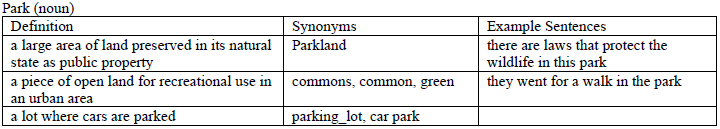
\includegraphics[width=5in]{figures/candidate-word-park-wordnet.png}
    \caption{Candidate word senses for the word \textit{park} from the WordNet database}
    \label{fig:candidate-word-park-wordnet}
\end{figure}

\subsection{Word sense disambiguation}

Using the information provided in WordNet, it is possible to perform word sense disambiguation. For a word in the schema and the metadata tags, we create a context using surrounding information available in the metadata. Similarly, we create a context for a word sense using the synonyms and the example sentences. After creating the contexts, we are able to compare the word with each candidate word sense using their contexts. If the two contexts are highly similar, then the metadata word is semantically enriched by attaching the definition of the word sense. 

\begin{figure}
    \centering
    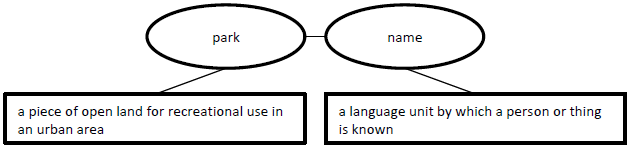
\includegraphics[width=5in]{figures/semantically-enriched-attribute.png}
    \caption{Semantically enriched attribute}
    \label{fig:semantically-enriched-attribute}
\end{figure}

While creating the contexts for the words and word senses, we do not add every word in the surrounding information to each context, since most of these words do not contribute to disambiguating word sense. For example, a sentence in the surrounding information can contain nouns, verbs, adjectives, prepositions, etc. We use part-of-speech tagging by the Hidden Markov Model to identify a word in a sentence as a noun, verb, etc. To simplify our work, we only add noun words to the context; we argue that nouns can contribute the most to word sense disambiguation. Each context therefore consists of a set of nouns. We then choose the word sense that has the most number context word overlaps.

The overlapping of words between two contexts is also known as the gloss overlap. Gloss overlaps increases the chance of finding similarities between contexts, since related contexts tend to contain many common words. Finding the similarity by using gloss overlaps is known as the Lesk method. By using the Lesk method, we perform syntax-driven semantic analysis, where the context words are just items in a collection and we count how many items are overlapping.

Once we disambiguate the word, we attach the definition to the word. We name the step to attach definitions to words in metadata as semantic enrichment. The words in the attributes of a schema and in the tags are semantically enriched. An example of a semantically enriched schema attribute, \textit{park name}, is shown in \autoref{fig:semantically-enriched-attribute}.

We provide an example of semantic enrichment next. Using the metadata of \autoref{fig:example-parks}, we create the context of the word \textit{park} using \textit{table description}, \textit{category}, and \textit{tags}. Similarly, for each candidate word sense of \textit{park} in \autoref{fig:candidate-word-park-wordnet}, we use the \textit{definition}, the \textit{synonyms}, and \textit{example sentences} to create the context. After performing part-of-speech tagging for the \textit{table description}, the \textit{category}, and the \textit{tags}, we collect all the nouns into a list, which serves as the context for the tag word park. Similarly, the nouns from the definition, the synonyms, and the example sentences are collected into a list, which serves as the context of each candidate word sense. The contexts for \textit{park} as well as all candidate word senses are shown in \autoref{fig:contexts-park-candidate}.

To compare between the tag word context and the word sense contexts, we find the number of overlapping items between each pair of sets. After stemming each word in each context, the number of overlapping items between \textit{park} and \textit{candidate word sense 1} is 1, for \textit{candidate word sense 2} it is 2, and for \textit{candidate word sense 3} it is 0. Therefore we select word sense \textit{candidate word sense 2}, to semantically enrich the tag word \textit{park} in \autoref{fig:example-parks}. Each semantically enriched tag is now called a topic.

\begin{figure}
    \centering
    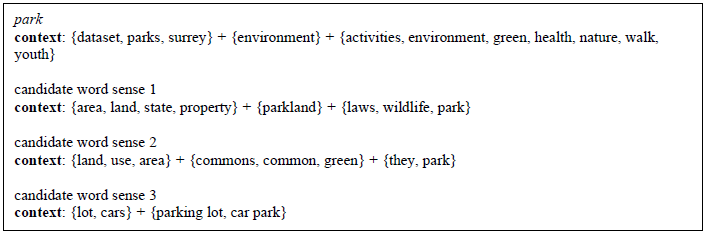
\includegraphics[width=5in]{figures/contexts-park-candidate.png}
    \caption{Contexts for tag \textit{park} and candidate word senses}
    \label{fig:contexts-park-candidate}
\end{figure}

Semantic enrichment of words can be viewed as a metadata generation problem, where we identify distinct concepts. When each concept consists of a group of words that have similar meanings, we are able to find all words belonging to the same concept instantaneously.

\subsection{Solution to semantic heterogeneity: dictionaries}
\label{ssec:SolutionToSemanticHeterogeneityDdictionaries}

When two elements (either tags, attributes, or other types of data) are highly similar in meaning, but are represented with different words or phrases, we rely on external resources such as a domain dictionary to determine if the two elements are similar. Using the domain dictionary, we are able to find all synonyms of a word. Even if two words are not synonyms of each other, they may still be semantically related.

Since a word can have many senses, the WordNet dictionary is a database that stores synonyms for each word sense, the set of synonyms with the same sense is called a Synset. WordNet has a separate entry for each sense of a word (the example in \autoref{fig:candidate-word-park-wordnet} has three entries), and indicates which Synset the entry belongs in. It is then possible to compute the semantic distance between a pair of Synsets.

To quantify the distance between word senses, one approach is to let each word sense in the database be connected to its closely related senses by directed edges in a graph, representing semantic relations between them \cite{cruz2005role}. The types of relations include synonym, hypernym, hyponym, and antonym. Each type of relation has a specified weight, and each directed edge of the relation type is given the weight. The semantic distance between two word senses is computed by selecting the optimal path from all the candidate paths, after averaging the weights along each path.

For example, when we compare \textit{dog(feline mammal usually having thick soft fur and no ability to roar: domestic cats; wildcats)} with \textit{cat(a member of the genus Canis that has been domesticated by man since prehistoric times; occurs in many breeds)}, the similarity between the pair of values determined by WordNet's \textit{path similarity} function is 0.2.

Another way to calculate the distance with WordNet is to use the information content of the lowest common subsumer \cite{Resnik1970Using}. All the senses of all words are organized into a tree hierarchy. For example, the words \textit{skating park} and \textit{amusement park} are daughters of \textit{park}, and \textit{park} is the most immediate common ancestor between them, then \textit{park} is the lowest common subsumer. To calculate the distance between two words, one can estimate the probability of encountering the lowest common subsumer. For example, if there are a total of 100,000 occurrences of park with the same sense, then this number is used to calculate a probability value which becomes the distance between the two words.

%%%%%%%%%%%%%%%%%%%%%%%%%%%%%%%%%%%%%%%%%%%%%%%%%%%%%%%%%%%%%%%%%%%%%%
\section{Schema matching}
\label{sec:SchemaMatching}

In this section, we give a detailed explanation of schema matching and its extensions \cite{Sorrentino2011NORMS}. Schema matching is an algorithm that compare between a pair schemata, where attributes in one schema are compared to attributes of the second schema to find a matching. The match operator is widely used in many applications \cite{Dong2012Proceedings} \cite{Rahm2001Survey} \cite{10.1145/3183713.3183729}, and it is a valuable tool for metadata management. Schema matching takes a pair of schemata as input (i.e. two sets of attributes to be matched), and identifies a set of pairs of attributes between the two schemata that are similar according to some criteria. Each pair in the matching is in the form of (a,b,c), called a correspondence, where a is an attribute from the first schema, b is an attribute from the second schema, and c is a score for the pair of matched attributes according to some matching criteria.

More formally, let a correspondence be a triple:
\[
(A_{si},A_{s'j},c), \; \textrm{for} \; A_{si}\in A_{s} \; \textrm{and} \; A_{s'j}\in A_{s'},\text{and }s\neq s'
\]
where $c$ is the score in the range {[}0, 1{]}, and $c$ = 1 indicates a perfect correspondence between $A_{si}$ and $A_{s'j}$ . The comparison criterion between a pair of attributes could be equality, subsumption, overlap, etc.

We give a description of pairwise schema matching next. We first compare each attribute of the first schema to every attribute in the other schema. Based on a criterion (such as overlap of alphanumeric characters in the attribute names), we computed the similarity score between each pair of attributes. We then apply any matching constraints required to create correspondences between pairs of attributes. A user can choose to place different constraints, and these constraints are enforced during schema matching. One example of a constraint is that each correspondence must have a score above a threshold set by the user.

Another constraint frequently used in many existing schema matching algorithms is the one-to-one cardinality constraint on the correspondences, which enforces that once an attribute participates in a correspondence, it cannot participate in another correspondence. When such a constraint is enforced, the correspondence is a matching. A schema matching algorithm can use an existing algorithm for matching to enforce the one-to-one cardinality constraint. For example, it can resolve two or more pairs that conflict with each other by choosing the pair that is the most probable. Alternatively, all possible matchings can be enumerated, and the best matching is selected.

There are many possible ways to implement a schema matching algorithm. Typically, under the following assumptions, an algorithm can be implemented correctly:

\begin{itemize}
\item The cardinality constraint on correspondences between a pair of schemata is one-to-one. However, this constraint can be relaxed if needed
\item A schema is present for each table, which allows schema matching to be performed instead of matching the header rows
\item When a pair of attributes have a high score, they have a high similarity according to some matching criteria.	
\end{itemize}

When the scores computed is in the range of 0 and 1, we can model the score as the probability that the pair of attributes fulfill the specified criteria. Based on the probabilities, we can then rank all correspondences by their scores or compute other statistical measures.

We give an example using \autoref{fig:example-parks} and \autoref{fig:example-park-specimen-trees}. We let a pair of schemata be
\begin{quote}
    \textit{Parks(park\_name, location, service\_classification)}, and \\
    \textit{ParkSpecimenTrees(location, park, tree\_species)}.
\end{quote}

We perform matching between the two sets of attributes. We first compare \textit{Parks.park\_name} with \textit{ParkSpecimenTrees.location}, and then with \textit{ParkSpecimenTrees.park}, and so on. If we use the simple \textbf{\gls{matching criterion}}: find the proportion of overlapping characters, then the scores for the comparisons are 0.25, 0.67, and so on. If the one-to-one cardinality constraint is enforced, we must only choose one pair of attributes such that neither of the two attributes appear in other correspondences, and that the sum of the correspondence scores is maximized. In the example, the pairs of attributes chosen as the correspondences are
\begin{quote}
\textit{(Parks.park\_name, ParkSpecimenTrees.park, 0.67)}, \\
\textit{(Parks.location, ParkSpecimenTrees.location, 1.0)}, and \\
\textit{(Parks.service\_classification, ParkSpecimenTrees.tree\_species, 0.32)}.
\end{quote}
If the one-to-one cardinality constraint is relaxed, then the chosen correspondences are changed.

\subsection{Using schema matching on open data}
\label{ssec:UsingSchemaMatchingOnOpenData}

Schema matching does not necessarily have to operate only on attributes in schemata. We can use the algorithm to find a matching between two sets of tags or between any pair of set-like data. The two sets can even be heterogeneous, where one set contains attributes and another set contains tags.

Therefore a correspondence can also be a triple:
\[
(L_{si},L_{s'j},c), \; \textrm{for} \; L_{si}\in L_{s} \; \textrm{and} \; L_{s'j}\in L_{s'}, \; \textrm{and} \; s\neq s'
\]
where $c$ is the score in the range [0, 1], and $c$ = 1 indicates a perfect correspondence between $L_{si}$ and $L_{s'j}$ . Schema matching between pairs of attributes and pairs of tags follow the one-to-one cardinality constraint.

We can use schema matching to compare other types of data such as long sentence descriptions and schema structure \cite{Sorrentino2011NORMS}. In \cite{10.1145/1066157.1066283} \cite{Duchateau2009YAM}, metadata such as schema version and namespaces were used in schema matching. It is also possible to perform schema matching using the data values in data instances \cite{Rahm2001Survey}. In our work, we use schema matching to find matching between a set of attributes and a set of tags, which we call the semantic labeling. Each pair of attribute and topic is called a semantic label.

Let a semantic label be a triple: 
\[
(A_{si},L_{s'j},c), \; \textrm{for} \; A_{si}\in A_{s}\ \; \textrm{and} \; L_{s'j}\in L_{s}
\]
where $c$ is the score in the range {[}0, 1{]} and $c$ = 1 indicates a perfect labeling between $A_{si}$ and $L_{s'j}$.

The cardinality constraint on semantic labeling of attributes and topics is many-to-one (i.e. a topic can have many attributes). We did not enforce the one-to-one cardinality constraint, because the output matching is too restrictive. To implement schema matching between attributes and tags, we specifically consider three cases of the many-to-one cardinality constraint.

In the first case, an attribute may correspond to multiple tags. We disallow this case because when an attribute is labeled with too many tags, there will be too much computation in the subsequent step (within the table search algorithm) of the metadata augmentation algorithm. But when there are multiple tags that are synonyms of each other, an attribute should correspond to all of these tags. We deal with synonyms in the partitioning algorithm of metadata augmentation. In the second case, many attributes in one schema may correspond to one tag. We allow this case. When matching between attributes and tags, it is desirable to have a tag participating in multiple correspondences because we only have a limited number of tags. The third case is that a tag may correspond to many attributes, where each attribute is from a different schema. We allow this case because this cardinality constraint on correspondences will produce a mapping similar to the data integration scenario, where the mapping allows a uniform access to data in all data instances, which is similar to what we want to achieve as well. The many-to-many cardinality constraint cannot be enforced, as discussed in a data integration scenario, GLAV mappings is typically disallowed because there are too many possible candidates, finding the optimal mapping is intractable \cite{Ehrig2004QOM}.

\subsection{Variations of schema matching}
\label{ssec:VariationsOfSchemaMatching}

The minimum form of schema matching does not usually produce correspondences accurately. Many variations of the minimum form are possible. Different variations of schema matching can improve the speed of matching as well as the quality of the correspondences. The matching criteria can be changed to reflect the similarity of attributes more accurately. One can use any linguistic-based criterion to compare the names of attributes, or use constraint-based criterion to compare the properties of the attributes. In constraint-based matching, an average can be computed for value of a numerical column. Other statistical quantities can be computed with the goal of characterizing the data distribution of the column. The matching criterion then make comparisons between two attributes based on their data distributions. The work in \autoref{ssec:SupervisedLearningForSchemaLabeling} performed matching using constraint-based criteria.

In linguistic-based criteria, a dictionary or thesaurus can be used to find the semantic similarity. We explain our linguistic-based criteria using a dictionary. Suppose that the word sense (i.e. the definition) of each word in an attribute is known, then when attributes are compared, the definitions of the words are compared instead. If it is possible to find the semantic distance (a numeric quantity) between the word senses, then the semantic distance of the attributes can be computed. The attribute park name with its attached definitions is shown in \autoref{fig:semantically-enriched-attribute}.

We use the WordNet dictionary to retrieve the definition of words, and compute the semantic similarity between a pair of values using WordNet's built-in functions. The details have been explained in \autoref{ssec:SolutionToSemanticHeterogeneityDdictionaries}.

We can also compute the semantic similarity between two values using pre-trained word embedding vectors. Words in an attribute is encoded as word embedding vectors using FastText \cite{Mudgal2018Deep} \cite{Nargesian2018Table}, a variant of Word2Vec. A pair of vectors can be compared, and if two words are used under similar contexts, they should also have similar vectors. When comparing between two sequences of words, the distance between their vectors is computed.

The minimum form of schema matching used a matching criterion that counts the proportion of overlapping characters of attribute names. A more sophisticated criterion at the character level is an N-Gram distance function that computes the similarity between a pair of values \cite{loper-bird-2002-nltk}. Each value is transformed into a multiset of character n-grams. For example, we use the values \textit{`EastPark'} and \textit{`SouthPark'} to illustrate how to compute the similarity between them. The bigrams of \textit{`EastPark'} are \textit{[`Ea', `as', `st', `tP', `Pa', `ar', `rk']}, and the bigrams for \textit{`SouthPark'} are \textit{[`So', `ou', `ut', `th', `hP', `Pa', `ar', `rk']}. The similarity is the proportion of shared n-grams between the two values, given by:

\[
\frac{2\times \left|ngrams(value1)\bigcap ngrams(value2)\right|}{\left|ngrams(value1)\right|+\left|ngrams(value2)\right|}
\]

Between \textit{`EastPark'} and \textit{`SouthPark'}, there are 3 shared bigrams \textit{[`Pa', `ar', `rk']}. The similarity is therefore 6/15 = 0.4.

Another variation of schema matching is to perform matching at the instance level. Matching at the instance-level compares the data values in the data instances instead of only comparing the attributes. For tabular data instances, matching is done between the table values instead of the table headers, by comparing data values in table columns, with the goal of finding which data column pairs share the most values. Matching at the instance-level is known as \textit{entity matching}. The work in \cite{Mudgal2018Deep} used instance-level matching to determine whether or not a pair of attributes are in the same data domain. Works in \cite{Rahm2016Case} used natural language processing(NLP) and deep neural network(DNN) techniques to improve the ability to resolve values for entity matching. If precise matching is required, then each of the values needs to resolve to real-world entities (such as a concept in an ontology), a process called \textit{entity resolution}. In open data there is typically no real-world entity information provided \cite{books/sp/bellahsene11}, and therefore instance-level matching cannot not be performed with precision. A course-grained instance-level matching approach is to use document similarity measures (such as TF/IDF) \cite{Duchateau2009YAM}, by treating each column as a document (with values of a column aggregated into a single document). This approach performs poorly since individual values such as address of a place requires more efforts to identify, and therefore similarity between documents is typically low. 

One can also perform matching with a combination of matching criteria within the same algorithm \cite{Sorrentino2011NORMS}. If an instance-level matching criterion is used in addition to a schema-level matching criterion, the instance-level criterion can add additional evidence for choosing the best correspondences. The reason is that each schema matching criterion specializes at evaluating certain types of data, because each criterion has a distinct similarity function. For example, a criterion that counts the proportion of word overlaps in attribute names is likely to produce different similarity values than a criterion that computes the semantic distance between words using a dictionary.

There are two ways to combine different matching criteria within the same algorithm, \textit{composite} and \textit{hybrid}. Composite matching combines the output attribute pairs from multiple independent matchings by merging the different sets into one set. For example, the set of pairs from one matching (with some criterion) is combined with the set from another matching (with another criterion) by removing conflicting pairs. Hybrid matching uses multiple matching criteria within the same matching algorithm. For each pair of attributes compared, a score is computed using multiple matching criteria, and the two scores are combined. A typical way to combine the scores is to compute a weighted average, where the weights are provided before matching \cite{DBLP:journals/debu/ChenGHTD18}. The weights can be trained by linear regression \cite{Ehrig2004QOM} such that the more effective criterion is given a greater weight. Other variations of hybrid matching exist. In \cite{Giunchiglia2005Semantic}, a decision tree is trained over a number of matching criteria, where the next matching criterion to use is decided based on the score produced by a previous score. In \cite{Moawed2018Arabian}, a neural network is trained that maps attribute features to Euclidean space, the vectors in Euclidean space are compared to compute the similarity scores.

%%%%%%%%%%%%%%%%%%%%%%%%%%%%%%%%%%%%%%%%%%%%%%%%%%%%%%%%%%%%%%%%%%%%%%
\section{Semantic labeling}
\label{sec:SemanticLabeling}

Once the cardinality constraint is enforced in the schema matching algorithm, semantic labeling can be performed. A semantic labeling is a mapping between an attribute and a tag (the header to a column), indicating that the data in the column contains data in the topic's domain. To create the semantic labeling for one schema, we perform schema matching between an attribute of the schema and every tag, similar to the approach discussed in \cite{Dong2012Proceedings} \cite{Salakhutdinov2009Semantic}. The attribute-tag pairs in the match are added to the result set; we call each attribute-tag pair a semantic label. An example of semantic labeling is shown in \autoref{fig:example-semantic-labeling}.

\begin{figure}
    \centering
    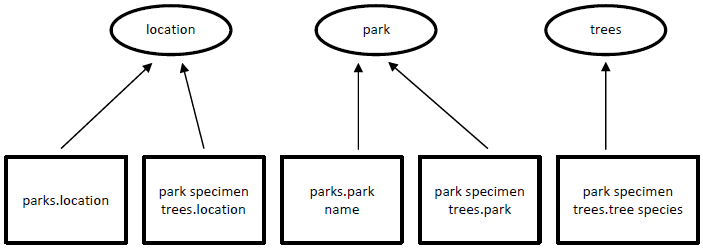
\includegraphics[width=5in]{figures/example-semantic-labeling.png}
    \caption{Example of a semantic labeling between attributes and tags.
    Each circle represents a tag, and each rectangle represents an attribute. There are two tables, \textit{parks} and \textit{park specimen trees}, each attribute of either table is mapped with a tag.}
    \label{fig:example-semantic-labeling}
\end{figure}

\subsection{Semantic labeling algorithm}
\label{ssec:SemanticLabelingAlgorithm}

For each text item $L_{sj}$ in the list of text items $L_{s}$ of data instance $s$, we add it to the set $L$. In our work, the text items are restricted to the tags. Then we perform schema matching between attributes $A_{s}$ and tags $L$, and according to the constraints defined in \autoref{ssec:UsingSchemaMatchingOnOpenData}, we create a semantic label $(A_{si},L_{s'j},c)$ for a pair of $A_{si}$ and $L_{s'j}$ with a high match score $c$. We use a threshold, and only add pairs with $c$ above the threshold and does not conflict with any existing constraints in schema matching. Since $s=s'$ or $s\neq s'$, there are $N$ or less semantic labels for $N$ attributes in a schema.

Suppose there is a tag $L_{sk}$ in the existing metadata of the data instance that does not participate in any semantic labels, we create a label $(null,L_{sk})$.

We give an example using \autoref{fig:example-parks} and \autoref{fig:example-drainage-catch-basins}. Let the input be the set of tags \textit{\{environment, green, nature, parks, trees, devices, infrastructure\}}, as well as a schema \textit{Parks(park name, location, service classification)}. The initialization step may generate the following semantic labels \textit{(park name, parks)}, \textit{(location, environment)}, \textit{(service classification, infrastructure)}. In addition, let another schema be \textit{DrainageCatchBasins(device type, device size)}, and the semantic labels be \textit{(device type, device)}, \textit{(device size, infrastructure)}.

Notice that both schemata have mappings to \textit{infrastructure}, but only one is suitable to contain this tag. The reason is because \textit{infrastructure} is used in different contexts in the two schemata. From the context of use, the word is more relevant to describe the structure built such as catch basins, rather than a service that may involve \textit{infrastructure}. In our main algorithm in \autoref{sec:IterativeApproach}, one of the two labels is not included in the result. We use the heuristic that \textit{DrainageCatchBasins} already contains the tag \textit{infrastructure} in its metadata, so it should keep the tag. In more complicated cases where neither tables contained the tag originally, it is more difficult to decide.

%%%%%%%%%%%%%%%%%%%%%%%%%%%%%%%%%%%%%%%%%%%%%%%%%%%%%%%%%%%%%%%%%%%%%%
\section{Finding relatedness between tables}
\label{sec:FindingRelatednessBetweenTables}

Normally, tables are related by foreign key constraints, but in open data there are usually no foreign key constraints that relate tables together. Given one table, it is difficult to select related tables because there is no guidance from the foreign key constraints. We therefore discuss an algorithm that searches the tables to find how tables are related. We first show how table search in \cite{Nargesian2018Table} works. Given a table as the query, the goal is to find tables (top-k) that are unionable by searching all tables in a repository. The measure of unionability is defined by the number of attribute pairs between two tables that store similar kinds of data, and therefore it is possible to merge the rows of these tables together by aligning the unionable attributes. To contrast, the joinability measure is defined by the number of attribute pairs that have some values that are the same.

\subsection{Table search on open data}
\label{ssec:TableSearchOnOpenData}

The table search algorithm relies on the schema matching algorithm. The query table is compared with every other table in a pairwise manner. For each pair of tables, a column in the first table is compared with every column in the second table. For each pair of column comparison, each value of the first column is compared with every value of the second column.

Three metrics are used to measure how similar two columns are: \textit{value overlap}, \textit{class overlap}, and \textit{natural language similarity}. The three metrics are three statistical tests to determine if a pair of columns are in the same data domain. The value overlap measure is based on the number of unique pairs of values that are the same between two columns. The class overlap additionally incorporates the semantic closeness of two values, it uses an ontology to find the distance between two values. When comparing between two sets, a hypothesis testing tests how likely the two sets, $A$ and $B$ are from the same domain $D$. The number of overlapping values, $t$, is calculated, and a cumulative distribution function is calculated over a hypergeometric distribution as follows:
\[
F(t|A,B) = \sum\limits _{0\le s\le t}\frac{C(n_{a},s)C(n_{D}-n_{a},n_{b}-s)}{C(n_{D},n_{b})}
\]
where C(a, b) is a combination a choose b. The natural language similarity first encodes each value into a fixed-dimension word embedding vector, which allows the comparison between two columns by the mean and variance of the vectors for the columns.

A similarity score for a pair of columns is computed from the three statistical tests performed, the score is called the \textit{attribute unionability}. After all pairs of columns are compared, all the attribute unionability scores are then used to perform schema matching. For the best matching between the two sets of attributes, a \textit{table unionability} score between the two tables is computed. For the given query table, it is then possible to find all other tables similar to the query table based on the unionability scores of tables.

Let the open data repository contain the tables in \autoref{fig:example-park-specimen-trees} and \autoref{fig:example-park-screen-trees}, \textit{park specimen trees} and \textit{park screen trees}. We compare the fourth column of \textit{park specimen trees}, $A$, with the third column of \textit{park screen trees}, $B$. Let $A={`rubrum', `rubrum', `nigra'}$ and $B={`japonica', `rubrum', `nigra', `nigra'}$. For the value overlap metric, the overlapping values shared is \textit{\{`rubrum', `nigra'\}}, thus $t=2$. Additionally, $n_D=|A+B|=7$, $n_A=|A|=3$, $n_B=|B|=4$. When $s=1$, the probability is computed by $C(4, 1) * C(4, 3) / C(7, 3)$. The cumulative function then sums up all probabilities of $s$ = 0 to $t$. However, due to both $A$ and $B$ being too large, computation of the probabilities requires hours, and requires further optimizations. The class overlap metric uses value similarities instead of value overlaps. The natural language similarity is computed using a vector representation for values, for example, when vector dimension is 3, one such vector is [0.2, 0.4, 0.4]. Let the three metrics computed be \{$m_o$, $m_v$, $m_n$\}. The attribute unionability is computed by averaging the three metrics.

Let the attribute unionability scores for the pairs of columns be \\ \{(\textit{ParkSpecimenTrees.park name} and \textit{ParkScreenTrees.location} : 0.2), (\textit{ParkSpecimenTrees.park name} and \textit{ParkScreenTrees.species} : 0.7), \dots\}. After a best matching is determined, let the table unionability be 0.4. When table search is performed with \textit{park specimen trees} as the query and the \textit{park screen trees} as a search candidate, they are unionable if 0.4 is above the decision threshold.

They relied on locality-sensitive hashing (LSH) to group all similar attributes from different tables into the same partition, which allows quick retrieval of all candidate tables containing an attribute similar to some given query attribute. However, building a LSH index takes a considerable amount of time, and depending on the problem, building such an index may not be desired.

\subsection{Modified table search}
\label{ssec:ModifiedTableSearch}

The table search algorithm discussed above does not assume any metadata other than the headers is available. We modify table search such that the tags will be utilized. Once semantic labeling is created for each table, we can perform table search by comparing pairs of semantic labels instead of comparing table columns. The attribute unionability score is omitted, and table unionability is defined as the number of overlapping tags (obtained from the semantic labels) between two tables. Table unionability is defined as $|L_{sq}\bigcap L_{s}|$. With one table $s_{q}$ as query, we find other tables $s\in D$ in the repository similar to the query table according to their table unionability scores. The tables $s\in D$ can then be ordered by their unionability scores.

Table search using the semantic labeling is a crude way to find the relatedness of tables, some tables may never be found while some irrelevant tables could appear to be related to the query. Even if the two tables do not share any common metadata tags, it is still possible that they are related. A semantic distance matching criterion can be used between tags instead of exact matches, since each tag are attached with its word definitions. Seemingly unrelated tables can then be related together by semantic similarity of their tags. Regarding the second question, additional tests can be performed once a table is found, to verify that it is indeed related.

%%%%%%%%%%%%%%%%%%%%%%%%%%%%%%%%%%%%%%%%%%%%%%%%%%%%%%%%%%%%%%%%%%%%%%
\section{Partitioning}
\label{sec:Partitioning}

Clustering is a common approach to group similar items together. In \cite{ilprints851}, a mediated schema is created by clustering of the attributes, where similar attributes are grouped into one group, and a mediated attribute is created for each group along with its schema mappings. The work in \cite{Smith2011Unity} also performed clustering before a topic is assigned to each cluster. The input to clustering is a set of attribute-to-attribute correspondences, represented as a graph, where the attributes are nodes and the pairwise similarity are the edges with a score as the edge weight. They then performed hierarchical clustering on the graph to discover clusters of attributes. For each cluster, they assigned a topic to each cluster, and then labeled each attribute in the cluster with that topic.

When semantic labeling is created for the attributes, clustering is a good choice for the tags only or the attributes only in the semantic labeling. However, if we want to discover groups based on the attributes-to-topics semantic labeling (with attributes and tags together), it is less clear how to perform clustering.

\subsection{Partitioning semantic labels}
\label{ssec:PartitioningSemanticLabels}

An alternative to clustering is partitioning. We describe an algorithm that partitions a set of semantic labels. The input to the algorithm is the semantic labeling between the attributes and tags from one or more tables. A number of partitions are created initially, the set of semantic labels $(A_{si},L_{s'j})$ of one table s is selected from the semantic labeling, and the tags $L_{s'j}$ in the semantic labels is used to create the initial partitions. Each partition is defined to be a tuple (\textit{Name},\textit{Sem-Lab},\textit{Attr-Set},\textit{Tag-Set}), where \textit{Name} is the name of the partition, \textit{Sem-Lab} is the set of semantic labels assigned to the partition, \textit{Attr-Set} is the set of attributes derived from the semantic labels, and \textit{Tag-Set} is the set of tags derived from the semantic labels. One partition is created for each tag in $L_{s'}$. The \textit{Name} for the partition is set to $L_{s'j}$, the semantic label $(A_{si},L_{s'j})$ is added to the \textit{Sem-Lab} set. Similarly, we add the attribute $A_{si}$ and the tag $L_{s'j}$ to \textit{Attr-Set} and \textit{Tag-Set} respectively. We note that $s$ is the table where $A_{si}$ originates from, and $s'$ is the table the tag $L_{s'j}$ originates from.

For the remaining semantic labels in the input, we add each label to the existing partitions by the following rules: when the tag is similar to most of the tags in \textit{Tag-Set} in one partition, and the attribute is similar to most of the attributes in \textit{Attr-Set} of the same partition, we add the tag, the attribute, and the semantic label to the partition. The similarity is a binary value, where a score above the threshold $\varphi$ for a proportion higher than $\mu$ is considered similar. We may also need to decide whether to place a semantic label in an existing partition or to create a new partition, by the following rules: when either the attribute is not similar to any of the \textit{Attr-Set} or the tag is not similar to any of the \textit{Tag-Set} of existing partitions, but there exists a partition where for both the attribute and the tag, the similarity is above a lower threshold $\varphi$ for a proportion higher than $\mu$. We then create a new partition using the semantic label.

To give an example, \textit{Parks} is the base table with semantic labeling \{(\textit{park name}, \textit{parks}), (\textit{location}, \textit{environment}), (\textit{service classification}, \textit{infrastructure})\}, we initialize partitions using the tags from these semantic labels. The partitions created are
\begin{quote}
(\textit{parks}, \{(\textit{Parks.park name}, \textit{parks})\}, \{\textit{Parks.park name}\}, \{\textit{parks}\}),
(\textit{environment}, \{(\textit{Parks.location}, \textit{environment})\}, \{\textit{Parks.location}\}, \{\textit{environment}\}), and
(\textit{infrastructure}, \{(\textit{Parks.service classification}, \textit{infrastructure})\}, \{\textit{Parks.service classification}\}, \{\textit{infrastructure}\}).
\end{quote}

Now consider the table \textit{ParkSpecimenTrees} with the semantic labeling \{(park, park)\}, the semantic label (\textit{park}, \textit{park}) will be added to the partition named park:
\begin{quote}
(\textit{parks}, \{(\textit{Parks.park name}, \textit{parks}), (\textit{ParkSpecimenTrees.park}, \textit{park})\}, \{\textit{Parks.park name}, \textit{ParkSpecimenTrees.park}\}, \{\textit{parks}, \textit{park}\})
\end{quote}

The partitioning algorithm may also take a set of unlabeled attributes as input. When there is no semantic label for an attribute, we cannot make tag comparisons, we can optionally compare with attributes in each partition only and add the attribute in the most similar existing partition. We also note that a semantic label can be added to multiple partitions if the similarity is high for all of these partitions, therefore the algorithm is not strictly performing partitioning.
\endinput